\subsection{Sformułowanie wymagań dotyczących dostępu do bazy i jej zawartości}
\begin{figure}[H]
    \centering
    \resizebox{0.8\columnwidth }{!}{%
    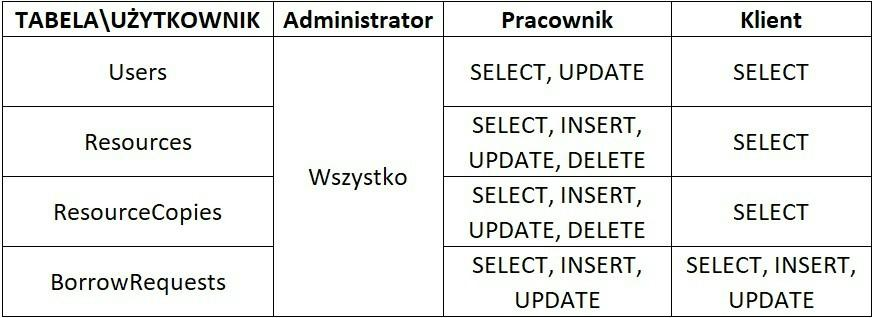
\includegraphics{Img/etap2IMG/1.png}%
    }
    \caption{Diagram wymagań dostępu do bazy i jej zawartości}
    %\label{}
\end{figure}
\subsection{Opracowanie diagramu modelu bazy na podstawie diagramu ERD}
\begin{figure}[H]
    \centering
    \resizebox{0.8\columnwidth }{!}{%
    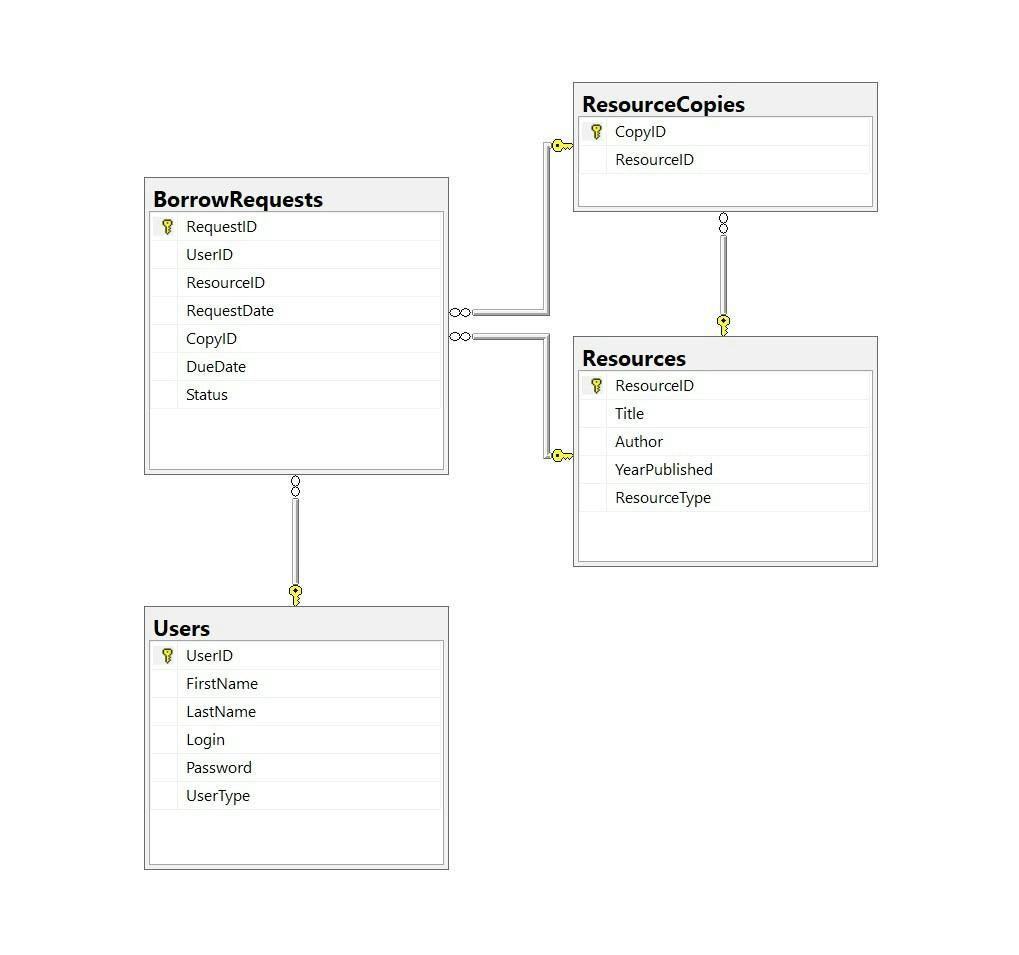
\includegraphics{Img/etap2IMG/2.png}%
    }
    \caption{Diagram modelu bazy danych}
    %\label{}
\end{figure}
\subsection{Model fizyczny bazy danych}

\subsubsection{Tabele}
\begin{minted}{tsql}
    CREATE TABLE Users (
    UserID INT PRIMARY KEY IDENTITY(1,1),
    FirstName VARCHAR(255) NOT NULL,
    LastName VARCHAR(255) NOT NULL,
    Login VARCHAR(255) UNIQUE NOT NULL,
    Password VARCHAR(255) NOT NULL,
    UserType VARCHAR(50) NOT NULL -- Client / Employee
    );

    GO

    CREATE TABLE Resources (
        ResourceID INT PRIMARY KEY IDENTITY(1,1),
        Title VARCHAR(255) NOT NULL,
        Author VARCHAR(255) NOT NULL,
        YearPublished INT NOT NULL,
        ResourceType VARCHAR(50) NOT NULL, -- Book / Magazine / ....
    );

    GO

    -- represents individual copies of resources
    CREATE TABLE ResourceCopies (
        CopyID INT PRIMARY KEY IDENTITY(1,1),
        ResourceID INT NOT NULL,
        FOREIGN KEY (ResourceID) REFERENCES Resources(ResourceID),
    );

    GO

    CREATE TABLE BorrowRequests (
        RequestID INT PRIMARY KEY IDENTITY(1,1),
        UserID INT NOT NULL,
        ResourceID INT NOT NULL,
        RequestDate DATE NOT NULL,
        CopyID INT, -- Assigned by Employee after acceptance
        DueDate DATE, -- Assigned by Employee after acceptance
        Status VARCHAR(50) NOT NULL, -- Pending / Approved / Returned
        FOREIGN KEY (UserID) REFERENCES Users(UserID),
        FOREIGN KEY (CopyID) REFERENCES ResourceCopies(CopyID),
        FOREIGN KEY (ResourceID) REFERENCES Resources(ResourceID),
    );

    GO
\end{minted}

\subsubsection{Widoki}
\begin{minted}{tsql}
    CREATE VIEW UserWithBorrowedResources AS
    SELECT
        U.UserID,
        R.ResourceID,
        R.Title,
        R.Author,
        R.YearPublished,
        R.ResourceType
    FROM Users U
    JOIN BorrowRequests BR ON U.UserID = BR.UserID
    JOIN ResourceCopies RC ON BR.CopyID = RC.CopyID
    JOIN Resources R ON BR.ResourceID = R.ResourceID
    WHERE BR.CopyID IS NOT NULL AND BR.Status <> 'Returned';
    GO

    CREATE VIEW SummarisedResources AS
    SELECT
        R.ResourceID,
        R.Title,
        COALESCE(RCTotal.TotalCopies, 0) AS TotalCopies,
        COALESCE(BRTotal.BorrowedCopies, 0) AS BorrowedCopies
    FROM Resources R
    LEFT JOIN (
        SELECT RC.ResourceID, COUNT(RC.CopyID) AS TotalCopies
        FROM ResourceCopies RC
        GROUP BY RC.ResourceID
    ) RCTotal ON R.ResourceID = RCTotal.ResourceID
    LEFT JOIN (
        SELECT BR.ResourceID, COUNT(DISTINCT BR.RequestID) AS BorrowedCopies
        FROM BorrowRequests BR
        WHERE BR.Status IN ('Approved', 'Pending') AND BR.CopyID IS NOT NULL
        GROUP BY BR.ResourceID
    ) BRTotal ON R.ResourceID = BRTotal.ResourceID;
    GO

    CREATE VIEW UserDetailsWithBorrowedResources AS
    SELECT
        U.UserID,
        U.FirstName,
        U.LastName,
        U.Login,
        U.UserType,
        BR.RequestID,
        BR.RequestDate,
        BR.CopyID,
        BR.DueDate,
        R.Title AS BorrowedResource
    FROM Users U
    JOIN BorrowRequests BR ON U.UserID = BR.UserID
    JOIN ResourceCopies RC ON BR.CopyID = RC.CopyID
    JOIN Resources R ON BR.ResourceID = R.ResourceID
    WHERE BR.Status = 'Approved';
    GO

    CREATE VIEW DelayedBorrowersView AS
    SELECT
        U.UserID,
        U.FirstName,
        U.LastName,
        BR.RequestID,
        R.Title AS BorrowedResource,
        BR.DueDate,
        DATEDIFF(DAY, BR.DueDate, GETDATE()) AS DaysLate
    FROM Users U
    JOIN BorrowRequests BR ON U.UserID = BR.UserID
    JOIN ResourceCopies RC ON BR.CopyID = RC.CopyID
    JOIN Resources R ON BR.ResourceID = R.ResourceID
    WHERE BR.Status = 'Returned' AND BR.DueDate < GETDATE();
    GO

    CREATE VIEW ApprovedBorrowRequests AS
    SELECT
        BR.RequestID,
        U.FirstName,
        U.LastName,
        R.Title AS BorrowedResource,
        BR.RequestDate,
        BR.DueDate,
        BR.Status
    FROM BorrowRequests BR
    JOIN Users U ON BR.UserID = U.UserID
    JOIN Resources R ON BR.ResourceID = R.ResourceID
    WHERE BR.Status = 'Approved';
    GO

    CREATE VIEW PendingBorrowRequests AS
    SELECT
        BR.RequestID,
        U.FirstName,
        U.LastName,
        R.Title AS RequestedResource,
        BR.RequestDate,
        BR.DueDate
    FROM BorrowRequests BR
    JOIN Users U ON BR.UserID = U.UserID
    JOIN Resources R ON BR.ResourceID = R.ResourceID
    WHERE BR.Status = 'Pending';
    GO
\end{minted}

\subsubsection{Przykładowe Dane}
\begin{minted}{tsql}
    -- Users
    INSERT INTO Users (FirstName, LastName, Login, Password, UserType) VALUES
    ('Adam', 'Nowak', 'anowak', 'pass123', 'Client'),
    ('Ewa', 'Kowalska', 'ekowalska', 'securepass', 'Client'),
    ('Mateusz', 'Wójcik', 'mwojcik', 'pass456', 'Client'),
    ('Karolina', 'Lis', 'klis', 'strongpass', 'Client'),
    ('Marcin', 'Kaczmarek', 'mkaczmarek', 'userpass', 'Client'),
    ('Alicja', 'Pawlak', 'apawlak', 'pass789', 'Client'),
    ('Michał', 'Duda', 'mduda', 'testpass', 'Client'),
    ('Katarzyna', 'Szymańska', 'kszymanska', 'mypassword', 'Client'),
    ('Piotr', 'Kowalczyk', 'pkowalczyk', 'pass1234', 'Client'),
    ('Anna', 'Jankowska', 'ajankowska', 'pass5678', 'Client'),
    ('Tomasz', 'Wiśniewski', 'twisniewski', 'securepass', 'Client'),
    ('Magdalena', 'Zając', 'mzajac', 'pass987', 'Client'),
    ('Grzegorz', 'Kowal', 'gkowal', 'testpass', 'Employee'),
    ('Agnieszka', 'Nowicka', 'anowicka', 'mypass', 'Employee'),
    ('Łukasz', 'Sikora', 'lsikora', 'pass654', 'Employee');

    GO

    -- Resources
    INSERT INTO Resources (Title, Author, YearPublished, ResourceType) VALUES
    ('Database Management', 'John Smith', 2020, 'Book'),
    ('Web Development Basics', 'Alice Johnson', 2019, 'Book'),
    ('Data Science in Practice', 'Michael Brown', 2022, 'Magazine'),
    ('Java Programming', 'Emily Davis', 2021, 'Book'),
    ('Introduction to Python', 'Daniel Wilson', 2018, 'Magazine'),
    ('Artificial Intelligence Fundamentals', 'Sophie White', 2020, 'Book'),
    ('Network Security', 'Andrew Miller', 2019, 'Book'),
    ('Software Engineering Principles', 'Olivia Taylor', 2022, 'Magazine'),
    ('Machine Learning Applications', 'William Brown', 2021, 'Book'),
    ('Mobile App Development', 'Emma Turner', 2018, 'Magazine');

    GO

    -- ResourceCopies
    INSERT INTO ResourceCopies (ResourceID) VALUES
    (1),
    (1),
    (1),
    (1),
    (1),
    (1),
    (1),
    (1),
    (1),
    (1),
    (1),
    (1),
    (2),
    (2),
    (2),
    (3),
    (3),
    (3),
    (4),
    (4),
    (4),
    (4),
    (4),
    (4),
    (4),
    (4),
    (4),
    (4),
    (4),
    (4),
    (4),
    (5),
    (5),
    (5),
    (5),
    (5),
    (5),
    (5),
    (5),
    (5),
    (5),
    (5),
    (5),
    (5),
    (5),
    (6),
    (6),
    (6),
    (6),
    (6),
    (6),
    (6),
    (6),
    (6),
    (6),
    (6),
    (6),
    (6),
    (6),
    (6),
    (6),
    (7),
    (7),
    (7),
    (8),
    (8),
    (8),
    (8),
    (8),
    (8),
    (8),
    (8),
    (8),
    (8),
    (8),
    (8),
    (9),
    (9),
    (9),
    (9),
    (9),
    (9),
    (9),
    (9),
    (9),
    (9),
    (9),
    (9),
    (9),
    (9),
    (9),
    (9),
    (9),
    (9),
    (10),
    (10),
    (10),
    (10),
    (10),
    (10),
    (10),
    (10),
    (10),
    (10),
    (10)
    GO

    -- BorrowRequest
    INSERT INTO BorrowRequests (UserID, ResourceID, RequestDate, CopyID, DueDate, Status) VALUES
    (1, 1, '2023-01-01', 1, '2023-01-15', 'Approved'),
    (3, 2, '2023-01-02',NULL, NULL, 'Pending'),
    (5, 3, '2023-01-03', NULL, NULL, 'Pending'),
    (2, 4, '2023-01-04', 4, '2024-01-15', 'Approved'),
    (4, 5, '2023-01-05', 5, '2023-01-20', 'Returned'),
    (6, 6, '2023-01-06', 6, '2023-01-21', 'Approved'),
    (8, 7, '2023-01-07', NULL, NULL, 'Pending'),
    (10, 8, '2023-01-08', 11, '2024-01-26', 'Approved'),
    (7, 9, '2023-01-09', NULL, NULL, 'Pending'),
    (9, 10, '2023-01-10', 10, '2023-01-25', 'Approved'),
    (11, 1, '2023-01-11', 11, '2023-01-26', 'Returned'),
    (7, 2, '2023-01-12', NULL, NULL, 'Pending'),
    (9, 3, '2023-01-13', NULL, NULL, 'Pending'),
    (12, 4, '2023-01-14', 13, '2023-01-28', 'Approved'),
    (1, 5, '2023-01-15', 14, '2023-01-29', 'Approved'),
    (4, 6, '2023-01-16', 15, '2023-01-30', 'Returned'),
    (3, 7, '2023-01-17', 1, '2023-08-30', 'Approved'),
    (5, 8, '2023-01-18', NULL, NULL, 'Pending'),
    (4, 9, '2023-01-19', 17, '2023-02-01', 'Returned'),
    (1, 10, '2023-01-20', NULL, NULL, 'Pending');
\end{minted}

\subsubsection{Wdrożenie i przetestowanie bazy}

\textbf{Tabela Users}
\begin{figure}[H]
    \centering
    \resizebox{0.8\columnwidth }{!}{%
    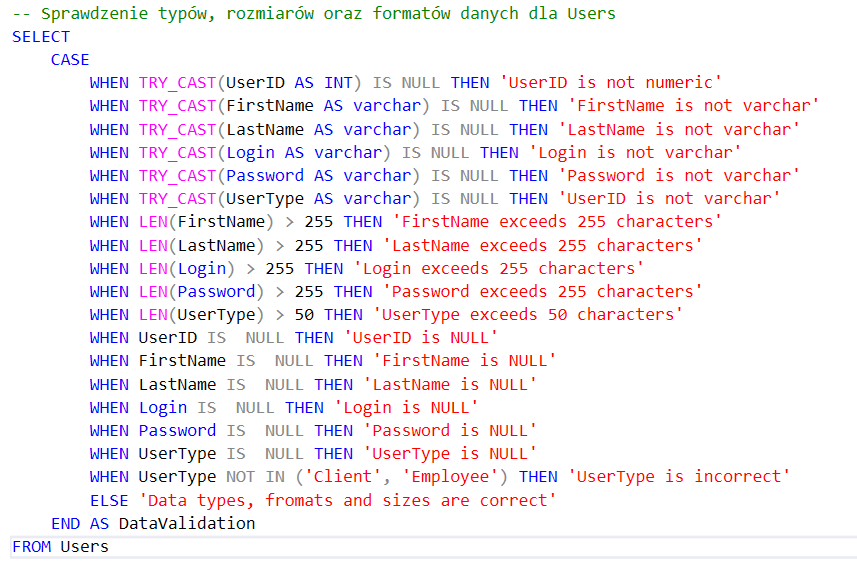
\includegraphics{Img/etap2IMG/9.png}%
    }
    \caption{Sprawdzenie integralności semantycznej- Kod}
    %\label{}
\end{figure}
\begin{figure}[H]
    \centering
    \resizebox{0.4\columnwidth }{!}{%
    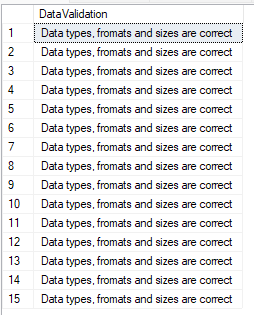
\includegraphics{Img/etap2IMG/10.png}%
    }
    \caption{Sprawdzenia integralności semantycznej - Wyniki}
    %\label{}
\end{figure}
\begin{figure}[H]
    \centering
    \resizebox{0.8\columnwidth }{!}{%
    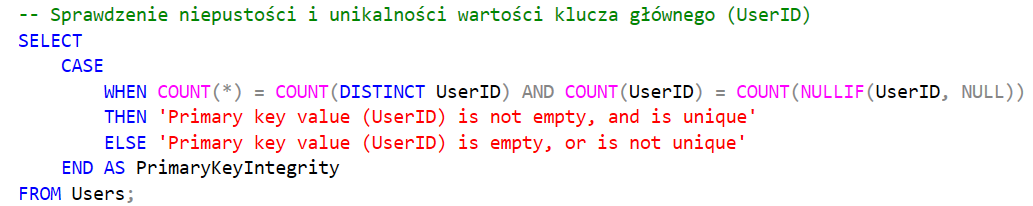
\includegraphics{Img/etap2IMG/11.5.png}%
    }
    \caption{Sprawdzenie integralności encji: - Kod}
    %\label{}
\end{figure}
\begin{figure}[H]
    \centering
    \resizebox{0.4\columnwidth }{!}{%
    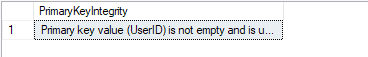
\includegraphics{Img/etap2IMG/11.png}%
    }
    \caption{Sprawdzenie integralności encji: - Wyniki}
    %\label{}
\end{figure}
\newpage
\textbf{Tabela Resources}
\begin{figure}[H]
    \centering
    \resizebox{0.8\columnwidth }{!}{%
    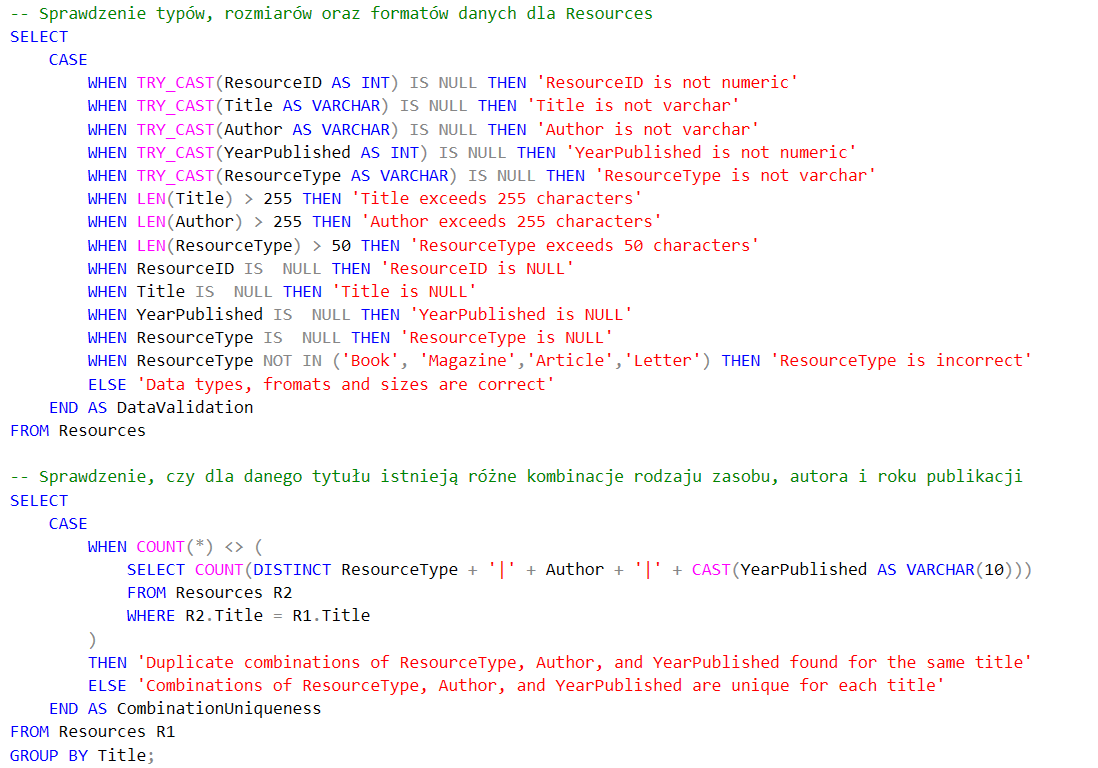
\includegraphics{Img/etap2IMG/12.png}%
    }
    \caption{Sprawdzenie integralności semantycznej- Kod}
    %\label{}
\end{figure}
\begin{figure}[H]
    \centering
    \resizebox{0.4\columnwidth }{!}{%
    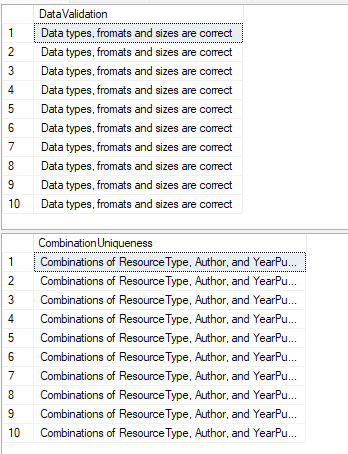
\includegraphics{Img/etap2IMG/13.png}%
    }
    \caption{Sprawdzenia integralności semantycznej - Wyniki}
    %\label{}
\end{figure}
\begin{figure}[H]
    \centering
    \resizebox{0.8\columnwidth }{!}{%
    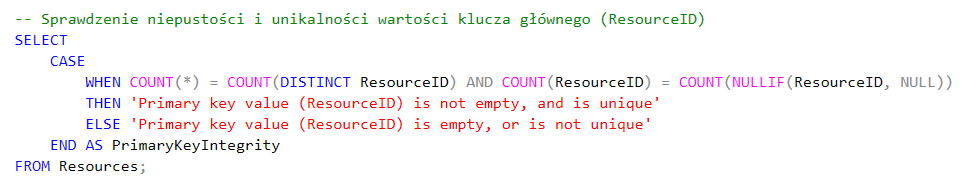
\includegraphics{Img/etap2IMG/14.png}%
    }
    \caption{Sprawdzenie integralności encji: - Kod}
    %\label{}
\end{figure}
\begin{figure}[H]
    \centering
    \resizebox{0.4\columnwidth }{!}{%
    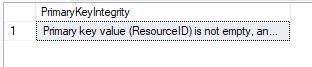
\includegraphics{Img/etap2IMG/15.png}%
    }
    \caption{Sprawdzenie integralności encji: - Wyniki}
    %\label{}
\end{figure}


\textbf{Tabela ResourcesCopies}
\begin{figure}[H]
    \centering
    \resizebox{0.8\columnwidth }{!}{%
    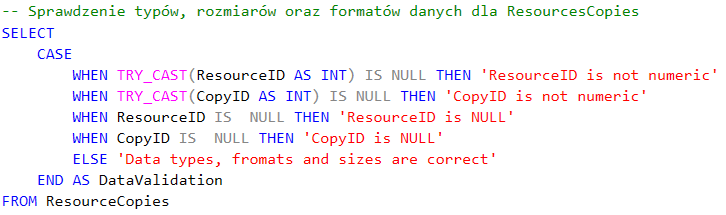
\includegraphics{Img/etap2IMG/16.png}%
    }
    \caption{Sprawdzenie integralności semantycznej- Kod}
    %\label{}
\end{figure}
\begin{figure}[H]
    \centering
    \resizebox{0.4\columnwidth }{!}{%
    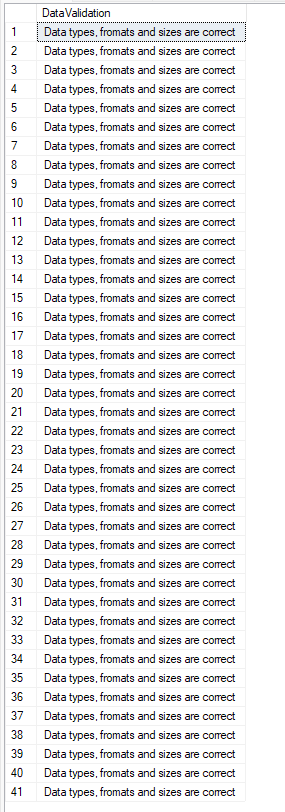
\includegraphics{Img/etap2IMG/17.png}%
    }
    \caption{Sprawdzenia integralności semantycznej - Wyniki}
    %\label{}
\end{figure}
\begin{figure}[H]
    \centering
    \resizebox{0.8\columnwidth }{!}{%
    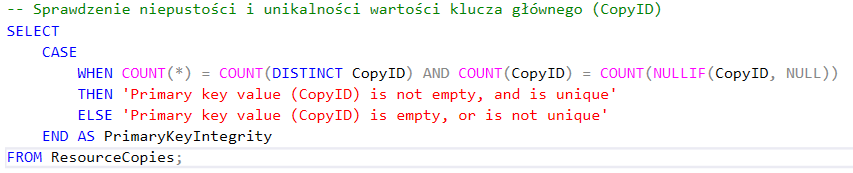
\includegraphics{Img/etap2IMG/18.png}%
    }
    \caption{Sprawdzenie integralności encji: - Kod}
    %\label{}
\end{figure}
\begin{figure}[H]
    \centering
    \resizebox{0.4\columnwidth }{!}{%
    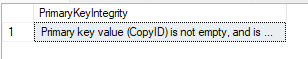
\includegraphics{Img/etap2IMG/19.png}%
    }
    \caption{Sprawdzenie integralności encji: - Wyniki}
    %\label{}
\end{figure}
\begin{figure}[H]
    \centering
    \resizebox{0.8\columnwidth }{!}{%
    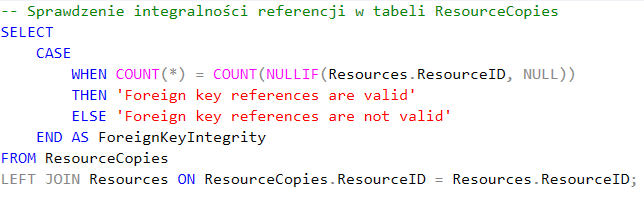
\includegraphics{Img/etap2IMG/20.png}%
    }
    \caption{Sprawdzenie integralności referencji: - Kod}
    %\label{}
\end{figure}
\begin{figure}[H]
    \centering
    \resizebox{0.4\columnwidth }{!}{%
    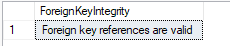
\includegraphics{Img/etap2IMG/21.png}%
    }
    \caption{Sprawdzenie integralności referencji: - Wyniki}
    %\label{}
\end{figure}

\newpage

\textbf{Tabela BorrowRequests}
\begin{figure}[H]
    \centering
    \resizebox{0.8\columnwidth }{!}{%
    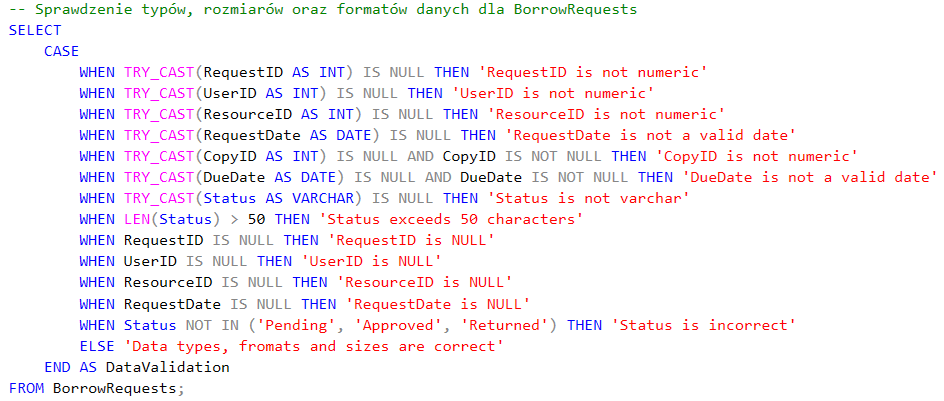
\includegraphics{Img/etap2IMG/22.png}%
    }
    \caption{Sprawdzenie integralności semantycznej- Kod}
    %\label{}
\end{figure}
\begin{figure}[H]
    \centering
    \resizebox{0.4\columnwidth }{!}{%
    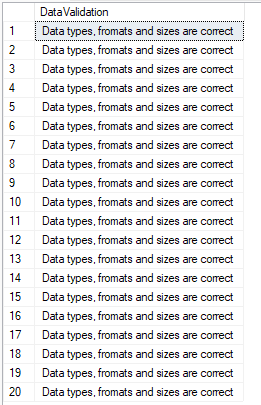
\includegraphics{Img/etap2IMG/23.png}%
    }
    \caption{Sprawdzenia integralności semantycznej - Wyniki}
    %\label{}
\end{figure}
\begin{figure}[H]
    \centering
    \resizebox{0.8\columnwidth }{!}{%
    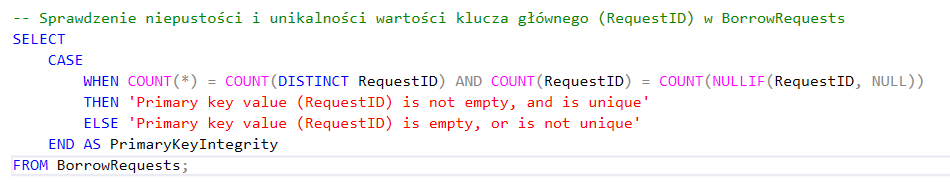
\includegraphics{Img/etap2IMG/24.png}%
    }
    \caption{Sprawdzenie integralności encji: - Kod}
    %\label{}
\end{figure}
\begin{figure}[H]
    \centering
    \resizebox{0.4\columnwidth }{!}{%
    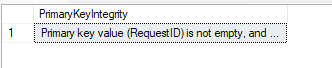
\includegraphics{Img/etap2IMG/25.png}%
    }
    \caption{Sprawdzenie integralności encji: - Wyniki}
    %\label{}
\end{figure}
\begin{figure}[H]
    \centering
    \resizebox{0.8\columnwidth }{!}{%
    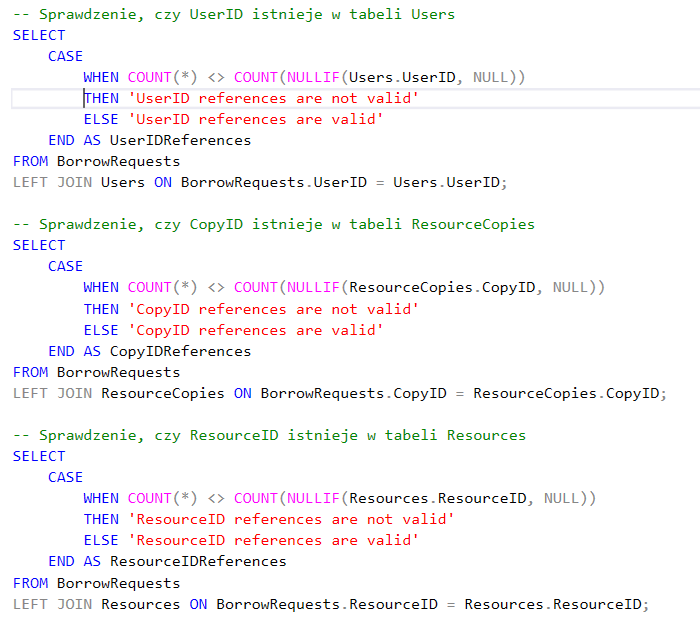
\includegraphics{Img/etap2IMG/26.png}%
    }
    \caption{Sprawdzenie integralności referencji: - Kod}
    %\label{}
\end{figure}
\begin{figure}[H]
    \centering
    \resizebox{0.4\columnwidth }{!}{%
    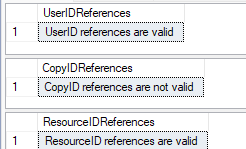
\includegraphics{Img/etap2IMG/27.png}%
    }
    \caption{Sprawdzenie integralności referencji: - Wyniki}
    %\label{}
\end{figure}